\documentclass[12pt]{article}\usepackage[]{graphicx}\usepackage[]{xcolor}
% maxwidth is the original width if it is less than linewidth
% otherwise use linewidth (to make sure the graphics do not exceed the margin)
\makeatletter
\def\maxwidth{ %
  \ifdim\Gin@nat@width>\linewidth
    \linewidth
  \else
    \Gin@nat@width
  \fi
}
\makeatother

\definecolor{fgcolor}{rgb}{0.345, 0.345, 0.345}
\newcommand{\hlnum}[1]{\textcolor[rgb]{0.686,0.059,0.569}{#1}}%
\newcommand{\hlsng}[1]{\textcolor[rgb]{0.192,0.494,0.8}{#1}}%
\newcommand{\hlcom}[1]{\textcolor[rgb]{0.678,0.584,0.686}{\textit{#1}}}%
\newcommand{\hlopt}[1]{\textcolor[rgb]{0,0,0}{#1}}%
\newcommand{\hldef}[1]{\textcolor[rgb]{0.345,0.345,0.345}{#1}}%
\newcommand{\hlkwa}[1]{\textcolor[rgb]{0.161,0.373,0.58}{\textbf{#1}}}%
\newcommand{\hlkwb}[1]{\textcolor[rgb]{0.69,0.353,0.396}{#1}}%
\newcommand{\hlkwc}[1]{\textcolor[rgb]{0.333,0.667,0.333}{#1}}%
\newcommand{\hlkwd}[1]{\textcolor[rgb]{0.737,0.353,0.396}{\textbf{#1}}}%
\let\hlipl\hlkwb

\usepackage{framed}
\makeatletter
\newenvironment{kframe}{%
 \def\at@end@of@kframe{}%
 \ifinner\ifhmode%
  \def\at@end@of@kframe{\end{minipage}}%
  \begin{minipage}{\columnwidth}%
 \fi\fi%
 \def\FrameCommand##1{\hskip\@totalleftmargin \hskip-\fboxsep
 \colorbox{shadecolor}{##1}\hskip-\fboxsep
     % There is no \\@totalrightmargin, so:
     \hskip-\linewidth \hskip-\@totalleftmargin \hskip\columnwidth}%
 \MakeFramed {\advance\hsize-\width
   \@totalleftmargin\z@ \linewidth\hsize
   \@setminipage}}%
 {\par\unskip\endMakeFramed%
 \at@end@of@kframe}
\makeatother

\definecolor{shadecolor}{rgb}{.97, .97, .97}
\definecolor{messagecolor}{rgb}{0, 0, 0}
\definecolor{warningcolor}{rgb}{1, 0, 1}
\definecolor{errorcolor}{rgb}{1, 0, 0}
\newenvironment{knitrout}{}{} % an empty environment to be redefined in TeX

\usepackage{alltt}

\usepackage{graphicx}
\usepackage{amsmath}
\usepackage[margin=1in]{geometry}
\usepackage{fancyhdr}
\usepackage{enumerate}
\usepackage[shortlabels]{enumitem}
\usepackage[spanish]{babel}
\usepackage{xurl}
\usepackage{tcolorbox}
\usepackage{titlesec}
\usepackage{listings}
\usepackage{xcolor}
\usepackage{pgfplots}
\usepackage{tikz}
\usepackage{cancel}
\usepackage[hidelinks]{hyperref}

\titleclass{\subsubsubsection}{straight}[\subsection]

\newcounter{subsubsubsection}[subsubsection]
\renewcommand\thesubsubsubsection{\thesubsubsection.\arabic{subsubsubsection}}
\renewcommand\theparagraph{\thesubsubsubsection.\arabic{paragraph}} % optional; useful if paragraphs are to be numbered

\titleformat{\subsubsubsection}
{\normalfont\normalsize\bfseries}{\thesubsubsubsection}{1em}{}
\titlespacing*{\subsubsubsection}
{0pt}{3.25ex plus 1ex minus .2ex}{1.5ex plus .2ex}

\makeatletter
\renewcommand\paragraph{\@startsection{paragraph}{5}{\z@}%
  {3.25ex \@plus1ex \@minus.2ex}%
  {-1em}%
  {\normalfont\normalsize\bfseries}}
\renewcommand\subparagraph{\@startsection{subparagraph}{6}{\parindent}%
  {3.25ex \@plus1ex \@minus .2ex}%
  {-1em}%
  {\normalfont\normalsize\bfseries}}
\def\toclevel@subsubsubsection{4}
\def\toclevel@paragraph{5}
% \def\toclevel@paragraph{6}
\def\toclevel@subparagraph{6}
\def\l@subsubsubsection{\@dottedtocline{4}{7em}{4em}}
\def\l@paragraph{\@dottedtocline{5}{10em}{5em}}
\def\l@subparagraph{\@dottedtocline{6}{14em}{6em}}
\makeatother

\setcounter{secnumdepth}{4}
\setcounter{tocdepth}{4}

% Set up headers and footers
\pagestyle{fancy}
\fancyhf{}  % Clear previous settings

\fancyhead[L]{Julián - Ludwig}
\fancyhead[C]{Taller 2 - Sim Estocástica}
\fancyhead[R]{\today}

\fancyfoot[C]{\thepage}
\fancyfoot[C]{\footnotesize Este trabajo está bajo una licencia CC BY-SA 4.0. Más info: \url{https://creativecommons.org/licenses/by/4.0/}}

\renewcommand{\headrulewidth}{0.2pt}


% Define R Style for listings
\lstdefinestyle{RStyle}{
  language=R,
  basicstyle=\ttfamily\small,
  keywordstyle=\color{blue}\bfseries,
  commentstyle=\color{green!40!black}\itshape,
  stringstyle=\color{red!70!black},
  numbers=left,
  numberstyle=\tiny\color{gray},
  stepnumber=1,
  numbersep=5pt,
  backgroundcolor=\color{gray!10},
  showstringspaces=false,
  breaklines=true,
  frame=single,
  rulecolor=\color{black},
  captionpos=b,
  morekeywords={generator}
}

% Set RStyle as default
\lstset{style=RStyle}
\IfFileExists{upquote.sty}{\usepackage{upquote}}{}
\begin{document}


\section{Stopping generating new simulation data}

Write a program to generate standard normal random variables until you have generated n of them, where $n \geq 100$ is such that $S/\sqrt{n} < 0.01$, where S is the sample standard deviation of the n data values. Note that this is the ``Method for Determining When to Stop Generating New Data''. Also, answer the following questions:



Debido a que se va a generar variables aleatorias \textbf{normales estándar} $X_{i}$, es decir, $X_{i} \sim \mathcal{N}(0, 1)$ y se debe parar de generar cuando $\frac{S}{\sqrt{n}} < 0.01$.

\begin{knitrout}
\definecolor{shadecolor}{rgb}{0.969, 0.969, 0.969}\color{fgcolor}\begin{kframe}
\begin{alltt}
\hldef{x} \hlkwb{<-} \hlkwd{numeric}\hldef{()}
\hldef{s} \hlkwb{<-} \hlnum{1}
\hldef{n} \hlkwb{<-} \hlnum{0}

\hlkwa{while}\hldef{(n} \hlopt{<} \hlnum{100} \hlopt{||} \hldef{s} \hlopt{/} \hlkwd{sqrt}\hldef{(n)} \hlopt{>=} \hlnum{0.01}\hldef{) \{}
  \hldef{x} \hlkwb{<-} \hlkwd{c}\hldef{(x,} \hlkwd{rnorm}\hldef{(}\hlnum{1}\hldef{))}
  \hldef{n} \hlkwb{<-} \hlkwd{length}\hldef{(x)}
  \hldef{s} \hlkwb{<-} \hlkwd{sd}\hldef{(x)}
\hldef{\}}

\hlkwd{cat}\hldef{(}\hlsng{"Cantidad de Xi generados"}\hldef{, n,} \hlsng{"\textbackslash{}n"}\hldef{)}
\end{alltt}
\begin{verbatim}
## Cantidad de Xi generados 10193
\end{verbatim}
\begin{alltt}
\hlkwd{cat}\hldef{(}\hlsng{"Desviación estándar"}\hldef{,} \hlkwd{round}\hldef{(s,} \hlnum{5}\hldef{),} \hlsng{"\textbackslash{}n"}\hldef{)}
\end{alltt}
\begin{verbatim}
## Desviación estándar 1.0096
\end{verbatim}
\begin{alltt}
\hlkwd{cat}\hldef{(}\hlsng{"Error estándar S/sqrt(n)"}\hldef{,} \hlkwd{round}\hldef{(s}\hlopt{/}\hlkwd{sqrt}\hldef{(n),} \hlnum{5}\hldef{),} \hlsng{"\textbackslash{}n"}\hldef{)}
\end{alltt}
\begin{verbatim}
## Error estándar S/sqrt(n) 0.01
\end{verbatim}
\end{kframe}
\end{knitrout}


En el código se declara una variable $s$ inicializada en 1 para que luego sea nuevamente computada a la desviación estándar de $x$ que es un vector que va a almacenar todas las variables normales aleatorias generadas. Según el enunciado tenemos una condición de que al menos deben haber 100 variables aleatorias generadas ($n \geq 100$) y que el error estándar sea menor a 0.01 ($S / \sqrt{n} < 0.01$). En el ciclo \lstinline|while|, por lo tanto, tiene sentido que el ciclo continue si alguna de las afirmaciones anteriores son falsas, por eso queda la condición de esa manera. Se hace uso de la función \lstinline|rnorm(1)| para que genere una variable aleatoria normal con los valores por defecto (promedio 0 y desviación 1). 






\subsection{How many normals do you think will be generated? Give an analytic estimate.}
\label{subsec:p1-a}

\subsubsection{Respuesta}

Aunque ya se tengan los resultados de la simulación, se puede hacer un estimado analítico con la condición $S / \sqrt{n} < 0.01$ donde se puede despejar $n$ para saber cuántas variables se necesitan para parar el criterio.

Se tiene en primer lugar la inecuación:

\[
\frac{S}{\sqrt{n}} < 0.01
\]

Se eleva ambas partes con menos 1:

\begin{align*}
  \left(\frac{S}{\sqrt{n}}  \right)^{-1} &> 0.01^{-1} \\
  \frac{\sqrt{n}}{S}  &> 100
\end{align*}

Multiplicando ambas partes por $S$:

\begin{align*}
  \cancel{S} \times \frac{\sqrt{n}}{\cancel{S}}  &> 100 \times S \\
  \sqrt{n} &> 100 \times S 
\end{align*}

Ahora se cancela la raíz elevando ambas partes al cuadrado:

\begin{align*}
  (\cancel{\sqrt{n}})^{\cancel{2}} &> (100 \times S)^{2} 
\end{align*}

Quedando entonces:

\[
n > 10000\times S^{2}
\]

Para hacer el ejercicio se utilizó en \textsf{R} la función \texttt{rnorm(1, mean = 0, sd = 1)}, de esta manera genera únicamente 1 valor con media 0 y desviación 1, por lo tanto, podemos hacer $S = 1$ para estimar cuántos $n$ necesitamos para que se cumpla condición y deje de generar variables aleatorias, por lo tanto:

\begin{align*}
  n &> 10000 \times (1)^{2} \\
  n &> 10000 
\end{align*}

Este valor se acerca bastante al que se imprime en la simulación. 











\subsection{How many normals did you generate?}
\label{subsec:p1-b}

\subsubsection{Respuesta}

Se han generado \lstinline|n=| $10193$ normales.


\subsection{What is the sample mean of all the normals generated?}
\label{subsec:p1-c}




\subsubsection{Respuesta}

Utilizando el comando \lstinline|mean()| al vector \lstinline|x| se obtiene $\ensuremath{6.0338234\times 10^{-4}}$. 

\subsection{What is the sample variance?}
\label{subsec:p1-d}


\subsubsection{Respuesta}

La varianza muestral se calcula como:

\[
S^{2} = \frac{\sum_{i=1}^{n} (X_{i} - \bar{X})^{2}}{n-1}
\]

Esto se puede sacar con la función \lstinline|var()| de \textsf{R}, por lo tanto, aplicando eso al vector \lstinline|x| se obtiene $1.0192875$.



\subsection{Comment on the results of (\ref{subsec:p1-c}) and (\ref{subsec:p1-d}). Were they surprising?}
\label{subsec:p1-e}

\subsubsection{Respuesta}

El resultado de \ref{subsec:p1-c} es la media de \lstinline|x| que es $\ensuremath{6.0338234\times 10^{-4}}$ y el de \ref{subsec:p1-d} es la varianza muestral de \lstinline|x| dando $1.0192875$. Estos valores muy sorprendentes no fueron... Se espera que al simular muchas veces una distribución normal, esta nos dé los valores de la media y la desviación estándar al cuadrado. Pero sí es interesante que dado este algoritmo para detenerse después de cruzar un $S / \sqrt{n}$ nos dé valores muy cercanos a una distribución normal con $\mu = 0$ y $\sigma = 1$.


\newpage

\section{Gaining confidence with confidence intervals}

We know that the $\mathcal{U}(-1, 1)$ r.v. has mean 0. Use a sample of size $1000$ to estimate the mean and give a $95\%$ confidence interval (CI). Does the CI contain 0? Repeat the above a large number of times ($\geq  100$). What percentage of time does the CI contain 0? Write your code so that it produces output similar to the following:

\begin{figure}[ht]
  \centering
  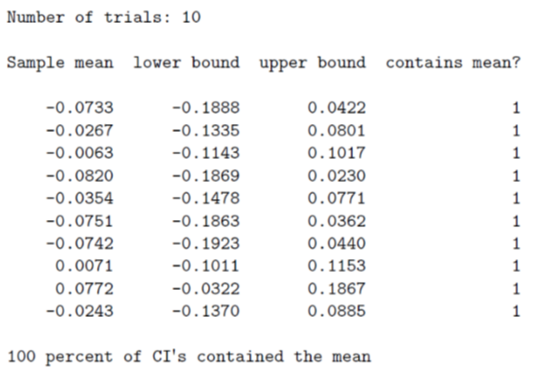
\includegraphics[width=0.6\textwidth]{img/Punto2.png}
\end{figure}

\subsection{Respuesta}

Se sabe que para tener un intervalo de confianza de 95\%, el límite inferior y superior serán, respectivamente:

\[
\left( \bar{X} - 1.96 \frac{S}{\sqrt{n}}, \bar{X} + 1.96 \frac{S}{\sqrt{n}} \right)
\]

El siguiente código permite sacar el intervalo de confianza del 95\% y también el estimado de la media.

\begin{knitrout}
\definecolor{shadecolor}{rgb}{0.969, 0.969, 0.969}\color{fgcolor}\begin{kframe}
\begin{alltt}
\hldef{n} \hlkwb{<-} \hlnum{1000}
\hldef{x} \hlkwb{<-} \hlkwd{runif}\hldef{(n,} \hlopt{-}\hlnum{1}\hldef{,} \hlnum{1}\hldef{)}
\hldef{xmean} \hlkwb{<-} \hlkwd{mean}\hldef{(x)}
\hldef{S} \hlkwb{<-} \hlkwd{sd}\hldef{(x)}
\hldef{L} \hlkwb{<-} \hldef{xmean} \hlopt{-} \hlnum{1.96} \hlopt{*} \hldef{S}\hlopt{/}\hlkwd{sqrt}\hldef{(n)}
\hldef{U} \hlkwb{<-} \hldef{xmean} \hlopt{+} \hlnum{1.96} \hlopt{*} \hldef{S}\hlopt{/}\hlkwd{sqrt}\hldef{(n)}
\hlkwd{cat}\hldef{(}\hlsng{"El estimado es"}\hldef{, xmean,} \hlsng{"\textbackslash{}n"}\hldef{)}
\end{alltt}
\begin{verbatim}
## El estimado es -0.01342494
\end{verbatim}
\begin{alltt}
\hlkwd{cat}\hldef{(}\hlsng{"95% está entre ("}\hldef{, L,} \hlsng{", "}\hldef{, U,} \hlsng{") \textbackslash{}n"}\hldef{,} \hlkwc{sep}\hldef{=}\hlsng{""}\hldef{)}
\end{alltt}
\begin{verbatim}
## 95% está entre (-0.04908598, 0.0222361)
\end{verbatim}
\end{kframe}
\end{knitrout}

Aquí se estimó la media de la distribución uniforme, dando un resultado de $-0.0134249$, muy cercano a 0. El intervalo de confianza está entre $-0.049086$ y $0.0222361$, en este caso sí contiene a 0.\footnote{Aquí hay que hacer una aclaración, los autores utilizaron \href{https://yihui.org/knitr/}{knitr}, una herramienta para la generación de reportes dinámicos en \textsf{R}, entonces cada vez que se compile este archivo \texttt{.Rnw} va a salir una salida diferente y puede ser que ya el intervalo no contenga 0.} Ahora, se va a realizar el proceso unas 200 veces para conocer el porcentaje de intervalos de confianza que contienen 0.

\begin{knitrout}
\definecolor{shadecolor}{rgb}{0.969, 0.969, 0.969}\color{fgcolor}\begin{kframe}
\begin{alltt}
\hldef{trials} \hlkwb{<-} \hlnum{200}
\hldef{n} \hlkwb{<-} \hlnum{1000}
\hldef{true_mean} \hlkwb{<-} \hlnum{0}

\hldef{results} \hlkwb{<-} \hlkwd{data.frame}\hldef{(}
  \hlkwc{sample_mean} \hldef{=} \hlkwd{numeric}\hldef{(trials),}
  \hlkwc{lower_bound} \hldef{=} \hlkwd{numeric}\hldef{(trials),}
  \hlkwc{upper_bound} \hldef{=} \hlkwd{numeric}\hldef{(trials),}
  \hlkwc{contains_mean} \hldef{=} \hlkwd{integer}\hldef{(trials)}
\hldef{)}

\hlkwa{for} \hldef{(i} \hlkwa{in} \hlnum{1}\hlopt{:}\hldef{trials)\{}
  \hldef{x} \hlkwb{<-} \hlkwd{runif}\hldef{(n,} \hlopt{-}\hlnum{1}\hldef{,} \hlnum{1}\hldef{)}
  \hldef{xmean} \hlkwb{<-} \hlkwd{mean}\hldef{(x)}
  \hldef{S} \hlkwb{<-} \hlkwd{sd}\hldef{(x)}
  \hldef{L} \hlkwb{<-} \hldef{xmean} \hlopt{-} \hlnum{1.96} \hlopt{*} \hldef{S}\hlopt{/}\hlkwd{sqrt}\hldef{(n)}
  \hldef{U} \hlkwb{<-} \hldef{xmean} \hlopt{+} \hlnum{1.96} \hlopt{*} \hldef{S}\hlopt{/}\hlkwd{sqrt}\hldef{(n)}
  \hldef{contains} \hlkwb{<-} \hlkwd{as.integer}\hldef{(L} \hlopt{<=} \hldef{true_mean} \hlopt{&} \hldef{true_mean} \hlopt{<=} \hldef{U)}

  \hldef{results[i, ]} \hlkwb{<-} \hlkwd{c}\hldef{(xmean, L, U, contains)}
\hldef{\}}

\hlkwd{cat}\hldef{(}\hlsng{"Número de intentos:"}\hldef{, trials,} \hlsng{"\textbackslash{}n"}\hldef{)}
\end{alltt}
\begin{verbatim}
## Número de intentos: 200
\end{verbatim}
\begin{alltt}
\hlkwd{print}\hldef{(results,} \hlkwc{digits}\hldef{=} \hlnum{4}\hldef{)}
\end{alltt}
\begin{verbatim}
##     sample_mean lower_bound upper_bound contains_mean
## 1    -1.985e-03   -0.037512   0.0335423             1
## 2     1.365e-02   -0.021017   0.0483215             1
## 3    -2.448e-03   -0.038018   0.0331216             1
## 4    -3.330e-02   -0.069442   0.0028334             1
## 5     1.970e-02   -0.015963   0.0553564             1
## 6    -9.186e-03   -0.045128   0.0267559             1
## 7    -1.068e-02   -0.046579   0.0252163             1
## 8     1.885e-04   -0.035480   0.0358575             1
## 9     6.076e-04   -0.033979   0.0351945             1
## 10    3.005e-02   -0.006450   0.0665501             1
## 11    1.361e-02   -0.022889   0.0501048             1
## 12   -1.751e-02   -0.053519   0.0184999             1
## 13   -1.091e-02   -0.046676   0.0248537             1
## 14    9.310e-03   -0.026271   0.0448898             1
## 15   -1.529e-02   -0.050931   0.0203431             1
## 16    3.968e-04   -0.034752   0.0355452             1
## 17   -6.167e-03   -0.041497   0.0291638             1
## 18   -2.625e-02   -0.061598   0.0091047             1
## 19    2.566e-02   -0.009728   0.0610581             1
## 20    1.530e-03   -0.032578   0.0356373             1
## 21   -6.948e-03   -0.042491   0.0285945             1
## 22    3.058e-03   -0.033229   0.0393441             1
## 23   -1.138e-02   -0.048329   0.0255716             1
## 24    2.282e-02   -0.011422   0.0570595             1
## 25   -1.114e-02   -0.046434   0.0241525             1
## 26   -2.348e-04   -0.036418   0.0359487             1
## 27    1.253e-02   -0.023374   0.0484430             1
## 28   -2.700e-02   -0.063069   0.0090705             1
## 29    5.519e-03   -0.030566   0.0416049             1
## 30   -3.466e-02   -0.070234   0.0009090             1
## 31   -3.064e-02   -0.066774   0.0054858             1
## 32   -1.703e-02   -0.053715   0.0196580             1
## 33   -3.392e-02   -0.070799   0.0029625             1
## 34    1.052e-02   -0.024567   0.0456093             1
## 35    9.200e-03   -0.027030   0.0454290             1
## 36    1.124e-02   -0.024207   0.0466888             1
## 37   -2.229e-02   -0.058399   0.0138225             1
## 38    2.198e-02   -0.013975   0.0579348             1
## 39   -7.682e-03   -0.042974   0.0276094             1
## 40   -3.676e-03   -0.039644   0.0322914             1
## 41   -8.066e-04   -0.037064   0.0354509             1
## 42    6.021e-03   -0.029869   0.0419114             1
## 43   -4.162e-03   -0.040450   0.0321275             1
## 44   -1.327e-02   -0.049119   0.0225890             1
## 45   -2.248e-02   -0.058635   0.0136666             1
## 46    2.629e-02   -0.008860   0.0614455             1
## 47    1.730e-03   -0.033502   0.0369628             1
## 48   -4.850e-03   -0.040003   0.0303021             1
## 49    1.786e-02   -0.017979   0.0537009             1
## 50    3.288e-02   -0.003493   0.0692474             1
## 51    9.923e-03   -0.026450   0.0462958             1
## 52    3.095e-03   -0.032832   0.0390232             1
## 53    1.474e-02   -0.020624   0.0501025             1
## 54   -3.420e-02   -0.070290   0.0018845             1
## 55   -5.365e-02   -0.089185  -0.0181153             0
## 56    3.252e-02   -0.003767   0.0688008             1
## 57   -2.401e-02   -0.059865   0.0118368             1
## 58   -1.274e-02   -0.048301   0.0228266             1
## 59   -3.401e-02   -0.069754   0.0017415             1
## 60    6.835e-03   -0.029354   0.0430234             1
## 61    2.123e-02   -0.014494   0.0569592             1
## 62    1.045e-02   -0.024438   0.0453294             1
## 63    4.857e-02    0.013386   0.0837568             0
## 64    1.404e-02   -0.022057   0.0501283             1
## 65    1.290e-02   -0.022932   0.0487286             1
## 66   -6.873e-03   -0.043428   0.0296829             1
## 67   -2.593e-02   -0.062114   0.0102557             1
## 68    7.951e-03   -0.028046   0.0439485             1
## 69   -1.444e-03   -0.037023   0.0341354             1
## 70    2.916e-02   -0.007384   0.0657084             1
## 71    1.261e-02   -0.023464   0.0486810             1
## 72   -3.352e-03   -0.039293   0.0325895             1
## 73    1.787e-02   -0.018324   0.0540537             1
## 74    2.495e-03   -0.033723   0.0387122             1
## 75    2.222e-03   -0.033887   0.0383307             1
## 76    2.123e-02   -0.014976   0.0574437             1
## 77   -1.826e-03   -0.036753   0.0331016             1
## 78    3.769e-02    0.002030   0.0733592             0
## 79   -1.555e-02   -0.051246   0.0201446             1
## 80    1.249e-02   -0.023048   0.0480378             1
## 81    5.937e-03   -0.029835   0.0417091             1
## 82   -7.996e-03   -0.043688   0.0276958             1
## 83   -2.713e-03   -0.038536   0.0331091             1
## 84   -1.343e-02   -0.048804   0.0219516             1
## 85   -7.346e-03   -0.042909   0.0282166             1
## 86   -1.551e-02   -0.051146   0.0201181             1
## 87   -2.773e-03   -0.037996   0.0324488             1
## 88   -1.492e-02   -0.050687   0.0208509             1
## 89    3.662e-03   -0.031690   0.0390140             1
## 90   -2.070e-02   -0.056869   0.0154704             1
## 91   -1.264e-02   -0.048860   0.0235702             1
## 92    7.436e-03   -0.028627   0.0434999             1
## 93   -1.221e-02   -0.047644   0.0232233             1
## 94   -5.682e-03   -0.042531   0.0311672             1
## 95   -2.748e-03   -0.038487   0.0329908             1
## 96    2.089e-02   -0.014753   0.0565417             1
## 97   -9.353e-03   -0.046227   0.0275214             1
## 98    6.608e-03   -0.030617   0.0438330             1
## 99   -1.443e-02   -0.050335   0.0214687             1
## 100  -2.812e-02   -0.063580   0.0073435             1
## 101   4.919e-02    0.013877   0.0845009             0
## 102  -1.992e-02   -0.055192   0.0153569             1
## 103  -3.283e-02   -0.067305   0.0016365             1
## 104  -5.362e-05   -0.036043   0.0359359             1
## 105  -6.268e-03   -0.041842   0.0293065             1
## 106  -2.381e-02   -0.059788   0.0121660             1
## 107   1.696e-02   -0.018260   0.0521752             1
## 108   1.836e-03   -0.033251   0.0369225             1
## 109  -1.052e-02   -0.046251   0.0252079             1
## 110  -1.221e-02   -0.048855   0.0244369             1
## 111   5.437e-03   -0.030962   0.0418371             1
## 112   9.785e-03   -0.025558   0.0451278             1
## 113  -1.208e-02   -0.048420   0.0242685             1
## 114   1.483e-02   -0.021456   0.0511150             1
## 115  -2.863e-02   -0.064448   0.0071917             1
## 116   1.442e-02   -0.022021   0.0508639             1
## 117  -8.382e-05   -0.036062   0.0358941             1
## 118  -1.333e-02   -0.049267   0.0226077             1
## 119   6.330e-03   -0.029396   0.0420567             1
## 120  -6.240e-04   -0.036785   0.0355372             1
## 121   3.312e-02   -0.001205   0.0674359             1
## 122   1.083e-02   -0.024291   0.0459503             1
## 123   1.382e-02   -0.021905   0.0495415             1
## 124  -9.549e-03   -0.044428   0.0253303             1
## 125  -2.036e-02   -0.056750   0.0160301             1
## 126  -2.753e-02   -0.063828   0.0087606             1
## 127   4.014e-02    0.004661   0.0756150             0
## 128   1.574e-02   -0.019963   0.0514470             1
## 129  -1.414e-02   -0.050377   0.0220897             1
## 130   5.342e-03   -0.030007   0.0406909             1
## 131  -2.593e-04   -0.035766   0.0352472             1
## 132  -4.338e-03   -0.040986   0.0323111             1
## 133  -6.000e-04   -0.036790   0.0355896             1
## 134   7.595e-03   -0.029166   0.0443559             1
## 135  -4.643e-03   -0.040464   0.0311770             1
## 136  -9.764e-03   -0.045158   0.0256301             1
## 137   2.752e-02   -0.008242   0.0632790             1
## 138   2.168e-02   -0.014203   0.0575564             1
## 139  -2.893e-02   -0.064702   0.0068390             1
## 140  -1.994e-02   -0.055252   0.0153724             1
## 141  -4.237e-03   -0.040395   0.0319216             1
## 142   3.325e-03   -0.032412   0.0390625             1
## 143  -1.907e-02   -0.055971   0.0178306             1
## 144  -2.825e-03   -0.039169   0.0335202             1
## 145  -1.403e-02   -0.049542   0.0214790             1
## 146  -6.187e-03   -0.041262   0.0288885             1
## 147  -2.320e-02   -0.058008   0.0116036             1
## 148  -2.075e-02   -0.056523   0.0150255             1
## 149   8.371e-03   -0.027176   0.0439177             1
## 150   1.168e-02   -0.023652   0.0470023             1
## 151   3.141e-03   -0.033557   0.0398401             1
## 152  -3.648e-02   -0.072078  -0.0008912             0
## 153   8.096e-03   -0.027369   0.0435611             1
## 154   1.245e-02   -0.024088   0.0489942             1
## 155  -1.712e-02   -0.053869   0.0196347             1
## 156  -2.392e-02   -0.059154   0.0113066             1
## 157  -2.327e-03   -0.038115   0.0334620             1
## 158  -3.019e-02   -0.065550   0.0051724             1
## 159   1.999e-02   -0.015648   0.0556280             1
## 160   1.025e-02   -0.025510   0.0460195             1
## 161   1.547e-02   -0.020499   0.0514306             1
## 162   3.022e-02   -0.006127   0.0665697             1
## 163   1.120e-02   -0.024098   0.0464890             1
## 164  -4.329e-04   -0.036336   0.0354698             1
## 165   2.039e-02   -0.014676   0.0554582             1
## 166   2.138e-02   -0.014722   0.0574750             1
## 167   1.898e-02   -0.016435   0.0544021             1
## 168   6.437e-03   -0.029099   0.0419719             1
## 169   3.106e-02   -0.004805   0.0669261             1
## 170  -1.680e-02   -0.052837   0.0192450             1
## 171   3.410e-03   -0.032970   0.0397899             1
## 172  -3.164e-02   -0.067978   0.0047003             1
## 173  -1.069e-02   -0.045104   0.0237173             1
## 174   4.775e-03   -0.031558   0.0411072             1
## 175  -4.980e-03   -0.040746   0.0307865             1
## 176   3.909e-02    0.003383   0.0748052             0
## 177  -7.578e-03   -0.043820   0.0286640             1
## 178   6.389e-03   -0.029922   0.0427007             1
## 179  -1.198e-02   -0.047783   0.0238165             1
## 180   3.330e-02   -0.001864   0.0684592             1
## 181   1.210e-02   -0.024091   0.0482820             1
## 182  -1.976e-02   -0.055389   0.0158772             1
## 183  -1.058e-02   -0.046091   0.0249338             1
## 184   1.071e-02   -0.024995   0.0464175             1
## 185   1.779e-02   -0.018011   0.0536012             1
## 186  -1.191e-02   -0.047275   0.0234599             1
## 187  -1.219e-02   -0.047987   0.0236100             1
## 188  -5.787e-04   -0.035431   0.0342738             1
## 189  -7.165e-03   -0.042356   0.0280253             1
## 190   2.625e-02   -0.009375   0.0618780             1
## 191   2.691e-03   -0.033738   0.0391214             1
## 192  -1.721e-02   -0.052907   0.0184776             1
## 193   1.026e-02   -0.025244   0.0457559             1
## 194  -1.226e-02   -0.047698   0.0231770             1
## 195  -2.120e-02   -0.057245   0.0148416             1
## 196   1.889e-02   -0.015408   0.0531858             1
## 197  -5.056e-03   -0.040653   0.0305415             1
## 198   1.311e-02   -0.023031   0.0492478             1
## 199   6.383e-03   -0.028482   0.0412480             1
## 200   1.974e-02   -0.015644   0.0551267             1
\end{verbatim}
\begin{alltt}
\hldef{porcentaje} \hlkwb{<-} \hlkwd{mean}\hldef{(results}\hlopt{$}\hldef{contains_mean)} \hlopt{*} \hlnum{100}

\hlkwd{cat}\hldef{(}\hlsng{"\textbackslash{}n"}\hldef{, porcentaje,} \hlsng{"% de los intervalos de"}\hldef{,}
\hlsng{"confianza contienen la media real\textbackslash{}n"}\hldef{)}
\end{alltt}
\begin{verbatim}
## 
##  96.5 % de los intervalos de confianza contienen la media real
\end{verbatim}
\end{kframe}
\end{knitrout}


En conclusión, el $96.5$ \% de los intervalos generados incluyen al 0.


\section{Standard deviation of a proportion}

Assume a manager is using the sample proportion $\hat{p}$ to estimate the proportion p of a new shipment of computer chips that are defective. He doesn’t know $p$ for this shipment, but in previous shipments it has been close to $0.01$, that is $1 \% $ of chips have been defective.

\subsection{If the manager wants the standard deviation of $\hat{p}$ to be about $0.02$, how large a sample should she take based on the assumption that the rate of defectives has not changed dramatically?}

En clase se vieron los estimadores de probabilidad, donde se quiere estimar

\[
  p = (P X \in A)
\]

Donde \(A\) es el subconjunto del espacio de estados de \(\Omega \) de \(X\). Es decir, para nuestro problema, este subconjunto de espacios en la muestra que tomó la administradora del cargamento de chips defectuosos. Se puede definir la variable indicadora \(Z\) como:

\[
  Z = 
  \begin{cases}
    1, & \quad X \in A \\
    0, & \quad X \notin A
  \end{cases}
\]

1 significa que sí está defectuoso y 0 que no lo está. Se puede escribir el estimador como:

\[
p = E[Z]
\]

En clase se realizó una demostración de como el valor esperado de \(Z\) se le puede asignar a \(p\). Se define la varianza de \(Z\) como:

\begin{align*}
\mathrm{Var}(Z) &= E[Z^{2}] - E[Z]^{2} \\
  &= (1^{2} \times P(X \in A) + 0^{2} \times P (X \notin A)) - (P(X \in A))^{²} \\
  &= p - p^{2}
\end{align*}

Aplicando factorización:

\[
\mathrm{Var}(Z) = p (1 - p)
\]

Estimar $p$ se puede realizar mediante el promedio muestral de $Z$, es decir, se puede estimar la proporción $\hat{p}$ con el promedio de los chips que son defectuosos:

\[
\hat{p} = \frac{1}{n} \sum_{i =1}^{n} Z_{i}
\]

Se puede calcular entonces, la varianza del estimador:

\[
\mathrm{Var}(\hat{p}) = \frac{1}{n} \mathrm{Var} \left(\sum_{i=1}^{n} Z_{i} \right)
\]

Por independencia de los valores del cargamento de chips $Z_{i}$ se puede meter la varianza de estos en la suma:

\begin{align*}
  \mathrm{Var}(\hat{p}) &= \frac{1}{n^{2}} \sum_{i=1}^{n} \mathrm{Var}(Z_{i}) \\
  &= \frac{1}{n^{2}} \sum_{i=1}^{n} p(1 - p) = \frac{1}{n} p (1 -p) 
\end{align*}

Por lo tanto, una aproximación es:

\[
\mathrm{Var}(\hat{p}) \approx \frac{1}{n} \hat{p} (1 - \hat{p}) 
\]

Teniendo en cuenta que la desviación estándar es el cuadrado de la varianza, se puede despejar:

\[
\sigma_{\hat{p}} \approx \sqrt{\frac{\hat{p} (1 - \hat{p})}{n}}
\]

El problema nos dice que la desviación estándar de $\hat{p}$ ($\sigma_{\hat{p}}$) debe ser sobre 0.02 y nos piden hallar cuántas muestras debe tomar la administradora, por lo tanto, en la parte izquierda de la ecuación reemplazamos por $0.02$, se despeja para $n$ y la proporción de defectuosos se toma como $0.01$ debido a que en el problema se nos dice que no ha cambiado tanto.

\begin{align*}
  \sigma_{\hat{p}} &\approx \sqrt{\frac{\hat{p} (1 - \hat{p})}{n}} \\
  0.02 &\approx \sqrt{\frac{0.1 (1 - 0.1)}{n}  } \\
  0.02 &\approx \sqrt{\frac{0.0099}{n}  } \\
  (0.02)^{2} &\approx \left(\cancel{\sqrt{\frac{0.0099}{n}  }} \right)^{\cancel{2}}\\
  0.0004 &\approx \frac{0.0099}{n} \\
  n &\approx \frac{0.0099}{0.0004} = 24.75
\end{align*}

Por lo tanto, la administradora debe tomar un muestra de por lo menos 25 chips para tener una desviación estándar de al menos $0.02$.

\subsection{Now suppose something went wrong with the production run and the actual proportion of defectives in the shipment is 0.3, that is 30 \% are defective. Now what would be the actual standard deviation of $\hat{p}$ for the sample size you choose in a)?}

Teniendo 25 chips y cambiando el valor de la proporción de defectuosos, se obtiene:

\begin{align*}
  \sigma_{\hat{p}} &\approx \sqrt{\frac{\hat{p}(1 - \hat{p}) }{n}} \\
                   &\approx   \sqrt{\frac{0.3(1 - 0.3) }{25}} \\
  &\approx 0.091
\end{align*}

Es decir, si la proporción de detección es del 30\%, la desviación estándar de $\hat{p}$ con una cantidad de chips de 25, será aproximadamente $0.091$.

\section{Bets}

You pay $10.000$ pesos to participate in a bet game, which consists in tossing two coins together. If two heads fall, you earn $15.000$ pesos. If one head and one tail fall you earn $5.000$ pesos. In any other case you earn nothing. Let $X$ the random variable of your profit.

\subsection{Analytically find the probability mass function $p_{X}$, the mean $E[X]$, and variance $\mathrm{Var}(X)$ of $X$.}

Dado que $X$ es la variable aleatoria de la ganancia, podemos listar los posibles valores que puede tomar de acuerdo a los lanzamientos:

\begin{table}[ht]
  \centering
  \begin{tabular}[h]{|c|c|c|c|}
    \hline
    \textbf{Salida moneda} & \textbf{Ganancia} & \textbf{Ganancia} $X$ & \textbf{Probabilidad} \\ \hline
    HH & $15.000$ & $+5.000$ & 0.25 \\ \hline
    HT-TH & $5.000$ & $-5.000$ & 0.5 \\ \hline
    TT & $0$ & $-10.000$ & 0.25 \\ \hline 
  \end{tabular}
  \caption{Posibles salidas y ganancias al tirar dos monedas, (H) cara y (T) sello.}
  \label{tab:p3}
\end{table}

Del cuadro \ref{tab:p3} se toma que los posibles valores para las ganancias son:

\[
X \in \{-5000, -10000, 5000  \} 
\]

La función de probabilida de masa: 

\[
p_{X} (x)  =
\begin{cases}
  0.25,& \quad x = 5000 \\
  0.5,&  \quad x = -5000 \\
  0.25,& \quad x = -10000 \\
  0,& \quad \text{En otro caso}
\end{cases}
\]

Para sacar el valor esperado se multiplica la probabilidad por cada valor de $X$:

\begin{gather*}
  E[X] = \sum_{I=1}^{3} x \dot p_{X}(x) = 5000(0.25) + (-5000)(0.5) + (-10000)(0.25) \\
  E[X] = 1250 - 2500 - 2500 = -3750
\end{gather*}

Es decir, en promedio se pierde $3.750$ pesos por jugada.

Para calcular la varianza se puede utilizar la fórmula:

\[
\mathrm{Var}(X) = E[X^{2}] - (E[X])^{2}
\]

Se computa $E[X^{2}]$:

\begin{align*}
  E[X^{2}] &= 5000^{2}(0.25) + (-5000)^{2}(0.5) + (-10000)^{2}(0.25) \\
           &= 25000000 (0.25) + 25000000 (0.5) + 100000000 (0.25) \\
  &= 6250000 + 12500000 + 25000000 = 43750000
\end{align*}

Ahora se le resta el cuadrado de la media:

\[
\mathrm{Var}(X) = 43750000 - (-3750)^{2} = 43750000 - 14062500 = 29687500
\]






\subsection{Write a code that simulates the r.v. \textbf{X} using the command sample. Generate an \textit{iid} \lstinline|sample| $\{X_{i}\}$ of size $n = 10^{5}$.}


\begin{knitrout}
\definecolor{shadecolor}{rgb}{0.969, 0.969, 0.969}\color{fgcolor}\begin{kframe}
\begin{alltt}
\hldef{outcomes} \hlkwb{<-} \hlkwd{c}\hldef{(}\hlopt{-}\hlnum{10000}\hldef{,} \hlopt{-}\hlnum{5000}\hldef{,} \hlnum{5000}\hldef{)}
\hldef{probabilities} \hlkwb{<-} \hlkwd{c}\hldef{(}\hlnum{0.25}\hldef{,} \hlnum{0.5}\hldef{,} \hlnum{0.25}\hldef{)}

\hldef{n} \hlkwb{<-} \hlnum{10}\hlopt{^}\hlnum{5}

\hldef{X} \hlkwb{<-} \hlkwd{sample}\hldef{(outcomes,} \hlkwc{size} \hldef{= n ,} \hlkwc{replace} \hldef{=} \hlnum{TRUE}\hldef{,} \hlkwc{prob} \hldef{= probabilities)}

\hlkwd{length}\hldef{(X)}
\end{alltt}
\begin{verbatim}
## [1] 100000
\end{verbatim}
\begin{alltt}
\hlkwd{summary}\hldef{(X)}
\end{alltt}
\begin{verbatim}
##    Min. 1st Qu.  Median    Mean 3rd Qu.    Max. 
##  -10000   -5000   -5000   -3728    5000    5000
\end{verbatim}
\end{kframe}
\end{knitrout}

En este fragmento de código se realiza la creación del vector \lstinline|X| de tamaño $10^{5}$ creado con la función \lstinline|sample| que toma las salidas que se explicaron anteriormente, el tamaño, que se reemplace y la probabilidad.


\subsection{Modify your code to calculate: (i) the estimated mean profit $\bar{X}_{j}$ for each sample subsequence: $\{X_{1}, X_{2}, . . . , X_{j} \}$, $j = 2, 3, \dots, n$, (ii) the $95 \%$ CI’s of each estimated mean profit $\bar{X}_{j}$ .}


\begin{knitrout}
\definecolor{shadecolor}{rgb}{0.969, 0.969, 0.969}\color{fgcolor}\begin{kframe}
\begin{alltt}
\hldef{mean_estimates} \hlkwb{<-} \hlkwd{numeric}\hldef{(n)}
\hldef{lower_CI} \hlkwb{<-} \hlkwd{numeric}\hldef{(n)}
\hldef{upper_CI} \hlkwb{<-} \hlkwd{numeric}\hldef{(n)}
\hldef{ie} \hlkwb{<-} \hlnum{1.96}

\hlkwa{for} \hldef{(j} \hlkwa{in} \hlnum{2}\hlopt{:}\hldef{n) \{}
  \hldef{x_sub} \hlkwb{<-} \hldef{X[}\hlnum{1}\hlopt{:}\hldef{j]}
  \hldef{mean_j} \hlkwb{<-} \hlkwd{mean}\hldef{(x_sub)}
  \hldef{sd_j} \hlkwb{<-} \hlkwd{sd}\hldef{(x_sub)}
  \hldef{se_j} \hlkwb{<-} \hldef{sd_j} \hlopt{/} \hlkwd{sqrt}\hldef{(j)}

  \hldef{mean_estimates[j]} \hlkwb{<-} \hldef{mean_j}
  \hldef{lower_CI[j]} \hlkwb{<-} \hldef{mean_j} \hlopt{-} \hldef{ie} \hlopt{*} \hldef{se_j}
  \hldef{upper_CI[j]} \hlkwb{<-} \hldef{mean_j} \hlopt{+} \hldef{ie} \hlopt{*} \hldef{se_j}
\hldef{\}}
\end{alltt}
\end{kframe}
\end{knitrout}

En esta parte del código se crean tres vectores \lstinline|mean_estimates|, \lstinline|lower_CI|, \lstinline|upper_CI| de tamaño $10^{5}$ y también una variable \lstinline|ie|. El bucle en cada iteración calcula la media muestral de los valores $\bar{X}_{j}$, la desviación estándar \lstinline|sd_j| y el error estándar, estos son necesarios para luego calcular el intervalo de confianza junto con la media.


\subsection{Plot $\bar{X}_{j}$ and their $95 \%$ CI’s in terms of $j = 2, \dots , 10^{5}$. Add an horizontal line corresponding to the actual value $E[X]$.}

\begin{knitrout}
\definecolor{shadecolor}{rgb}{0.969, 0.969, 0.969}\color{fgcolor}\begin{kframe}
\begin{alltt}
\hlcom{# Your plotting code remains the same}
\hlkwd{plot}\hldef{(}\hlnum{2}\hlopt{:}\hldef{n, mean_estimates[}\hlnum{2}\hlopt{:}\hldef{n],} \hlkwc{type} \hldef{=} \hlsng{"l"}\hldef{,} \hlkwc{col} \hldef{=} \hlsng{"blue"}\hldef{,} \hlkwc{lwd} \hldef{=} \hlnum{1}\hldef{,}
     \hlkwc{xlab} \hldef{=} \hlsng{"j (tamaño de la submuestra)"}\hldef{,}
     \hlkwc{ylab} \hldef{=} \hlsng{"Ganancia esperada estimada"}\hldef{,}
     \hlkwc{main} \hldef{=} \hlsng{"Evolución de la media muestral y su IC del 95%"}\hldef{)}
\hlkwd{lines}\hldef{(}\hlnum{2}\hlopt{:}\hldef{n, lower_CI[}\hlnum{2}\hlopt{:}\hldef{n],} \hlkwc{col} \hldef{=} \hlsng{"red"}\hldef{,} \hlkwc{lty} \hldef{=} \hlnum{2}\hldef{)}
\hlkwd{lines}\hldef{(}\hlnum{2}\hlopt{:}\hldef{n, upper_CI[}\hlnum{2}\hlopt{:}\hldef{n],} \hlkwc{col} \hldef{=} \hlsng{"red"}\hldef{,} \hlkwc{lty} \hldef{=} \hlnum{2}\hldef{)}
\hlkwd{abline}\hldef{(}\hlkwc{h} \hldef{=} \hlopt{-}\hlnum{3750}\hldef{,} \hlkwc{col} \hldef{=} \hlsng{"darkgreen"}\hldef{,} \hlkwc{lty} \hldef{=} \hlnum{3}\hldef{,} \hlkwc{lwd} \hldef{=} \hlnum{2}\hldef{)}
\hlkwd{legend}\hldef{(}\hlsng{"topright"}\hldef{,} \hlkwc{legend} \hldef{=} \hlkwd{c}\hldef{(}\hlsng{"Media estimada"}\hldef{,} \hlsng{"IC 95%"}\hldef{,} \hlsng{"Valor real E[X]"}\hldef{),}
       \hlkwc{col} \hldef{=} \hlkwd{c}\hldef{(}\hlsng{"blue"}\hldef{,} \hlsng{"red"}\hldef{,} \hlsng{"darkgreen"}\hldef{),} \hlkwc{lty} \hldef{=} \hlkwd{c}\hldef{(}\hlnum{1}\hldef{,} \hlnum{2}\hldef{,} \hlnum{3}\hldef{),} \hlkwc{bty} \hldef{=} \hlsng{"n"}\hldef{)}
\end{alltt}
\end{kframe}
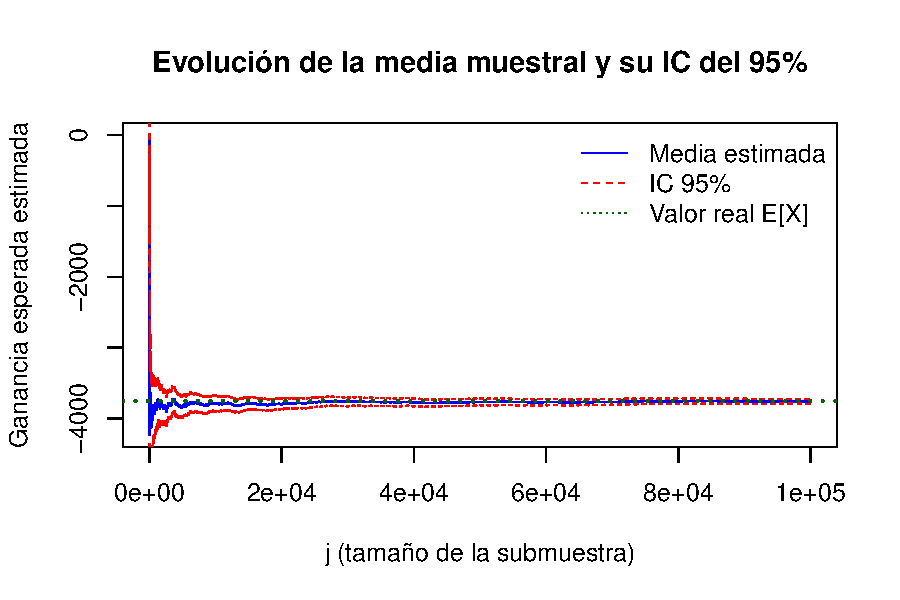
\includegraphics[width=\maxwidth]{figure/grafico-pdf-1} 
\end{knitrout}

Se puede ver que a medida que se aumenta la submuestra $j$, la media estimada $\bar{X}$ se acerca más al valor esperado $E[X]$ y también, el intervalo de confianza se va acortando más.




\subsection{Repeat \textit{c)} and \textit{d)} to estimate the probabilities $p_{X} (x)$, their $95 \%$ CI’s, and their plots for each $j = 2, \dots , 10^{5}$, adding the actual values.}



\begin{knitrout}
\definecolor{shadecolor}{rgb}{0.969, 0.969, 0.969}\color{fgcolor}\begin{kframe}
\begin{alltt}
\hlcom{# Posibles valores de X}
\hldef{outcomes} \hlkwb{<-} \hlkwd{c}\hldef{(}\hlopt{-}\hlnum{10000}\hldef{,} \hlopt{-}\hlnum{5000}\hldef{,} \hlnum{5000}\hldef{)}
\hldef{probs_true} \hlkwb{<-} \hlkwd{c}\hldef{(}\hlnum{0.25}\hldef{,} \hlnum{0.5}\hldef{,} \hlnum{0.25}\hldef{)}

\hlcom{# Inicializar matrices para almacenar las estimaciones y CIs}
\hldef{p_estimates} \hlkwb{<-} \hlkwd{matrix}\hldef{(}\hlnum{0}\hldef{,} \hlkwc{nrow} \hldef{= n,} \hlkwc{ncol} \hldef{=} \hlnum{3}\hldef{)}
\hldef{p_lower} \hlkwb{<-} \hlkwd{matrix}\hldef{(}\hlnum{0}\hldef{,} \hlkwc{nrow} \hldef{= n,} \hlkwc{ncol} \hldef{=} \hlnum{3}\hldef{)}
\hldef{p_upper} \hlkwb{<-} \hlkwd{matrix}\hldef{(}\hlnum{0}\hldef{,} \hlkwc{nrow} \hldef{= n,} \hlkwc{ncol} \hldef{=} \hlnum{3}\hldef{)}

\hldef{z} \hlkwb{<-} \hlnum{1.96}  \hlcom{# Nivel de confianza del 95%}

\hlkwa{for} \hldef{(j} \hlkwa{in} \hlnum{2}\hlopt{:}\hldef{n) \{}
  \hldef{x_sub} \hlkwb{<-} \hldef{X[}\hlnum{1}\hlopt{:}\hldef{j]}
  \hlkwa{for} \hldef{(i} \hlkwa{in} \hlnum{1}\hlopt{:}\hlnum{3}\hldef{) \{}
    \hldef{val} \hlkwb{<-} \hldef{outcomes[i]}
    \hldef{p_hat} \hlkwb{<-} \hlkwd{mean}\hldef{(x_sub} \hlopt{==} \hldef{val)}
    \hldef{se} \hlkwb{<-} \hlkwd{sqrt}\hldef{(p_hat} \hlopt{*} \hldef{(}\hlnum{1} \hlopt{-} \hldef{p_hat)} \hlopt{/} \hldef{j)}

    \hldef{p_estimates[j, i]} \hlkwb{<-} \hldef{p_hat}
    \hldef{p_lower[j, i]} \hlkwb{<-} \hlkwd{max}\hldef{(}\hlnum{0}\hldef{, p_hat} \hlopt{-} \hldef{z} \hlopt{*} \hldef{se)}
    \hldef{p_upper[j, i]} \hlkwb{<-} \hlkwd{min}\hldef{(}\hlnum{1}\hldef{, p_hat} \hlopt{+} \hldef{z} \hlopt{*} \hldef{se)}
  \hldef{\}}
\hldef{\}}
\end{alltt}
\end{kframe}
\end{knitrout}

\textbf{Gráfico de las probabilidades estimadas con sus ICs para cada posible valor de $X$:}

\begin{knitrout}
\definecolor{shadecolor}{rgb}{0.969, 0.969, 0.969}\color{fgcolor}\begin{kframe}
\begin{alltt}
\hldef{colors} \hlkwb{<-} \hlkwd{c}\hldef{(}\hlsng{"blue"}\hldef{,} \hlsng{"orange"}\hldef{,} \hlsng{"purple"}\hldef{)}
\hldef{labels} \hlkwb{<-} \hlkwd{c}\hldef{(}\hlsng{"p_X(-10000)"}\hldef{,} \hlsng{"p_X(-5000)"}\hldef{,} \hlsng{"p_X(5000)"}\hldef{)}
\hldef{true_values} \hlkwb{<-} \hlkwd{c}\hldef{(}\hlnum{0.25}\hldef{,} \hlnum{0.5}\hldef{,} \hlnum{0.25}\hldef{)}

\hlkwd{plot}\hldef{(}\hlnum{2}\hlopt{:}\hldef{n, p_estimates[}\hlnum{2}\hlopt{:}\hldef{n,}\hlnum{1}\hldef{],} \hlkwc{type} \hldef{=} \hlsng{"l"}\hldef{,} \hlkwc{col} \hldef{= colors[}\hlnum{1}\hldef{],} \hlkwc{ylim} \hldef{=} \hlkwd{c}\hldef{(}\hlnum{0}\hldef{,}\hlnum{1}\hldef{),}
     \hlkwc{xlab} \hldef{=} \hlsng{"j (tamaño de la submuestra)"}\hldef{,} \hlkwc{ylab} \hldef{=} \hlsng{"Probabilidad estimada"}\hldef{,}
     \hlkwc{main} \hldef{=} \hlsng{"Estimación de $p_X(x)$ con ICs del 95%"}\hldef{)}

\hlkwa{for} \hldef{(i} \hlkwa{in} \hlnum{1}\hlopt{:}\hlnum{3}\hldef{) \{}
  \hlkwd{lines}\hldef{(}\hlnum{2}\hlopt{:}\hldef{n, p_estimates[}\hlnum{2}\hlopt{:}\hldef{n,i],} \hlkwc{col} \hldef{= colors[i],} \hlkwc{lwd} \hldef{=} \hlnum{1}\hldef{)}
  \hlkwd{lines}\hldef{(}\hlnum{2}\hlopt{:}\hldef{n, p_lower[}\hlnum{2}\hlopt{:}\hldef{n,i],} \hlkwc{col} \hldef{= colors[i],} \hlkwc{lty} \hldef{=} \hlnum{2}\hldef{)}
  \hlkwd{lines}\hldef{(}\hlnum{2}\hlopt{:}\hldef{n, p_upper[}\hlnum{2}\hlopt{:}\hldef{n,i],} \hlkwc{col} \hldef{= colors[i],} \hlkwc{lty} \hldef{=} \hlnum{2}\hldef{)}
  \hlkwd{abline}\hldef{(}\hlkwc{h} \hldef{= true_values[i],} \hlkwc{col} \hldef{= colors[i],} \hlkwc{lty} \hldef{=} \hlnum{3}\hldef{,} \hlkwc{lwd} \hldef{=} \hlnum{1.5}\hldef{)}
\hldef{\}}

\hlkwd{legend}\hldef{(}\hlsng{"topright"}\hldef{,} \hlkwc{legend} \hldef{= labels,} \hlkwc{col} \hldef{= colors,} \hlkwc{lty} \hldef{=} \hlnum{1}\hlopt{:}\hlnum{1}\hldef{,} \hlkwc{bty} \hldef{=} \hlsng{"n"}\hldef{)}
\end{alltt}
\end{kframe}
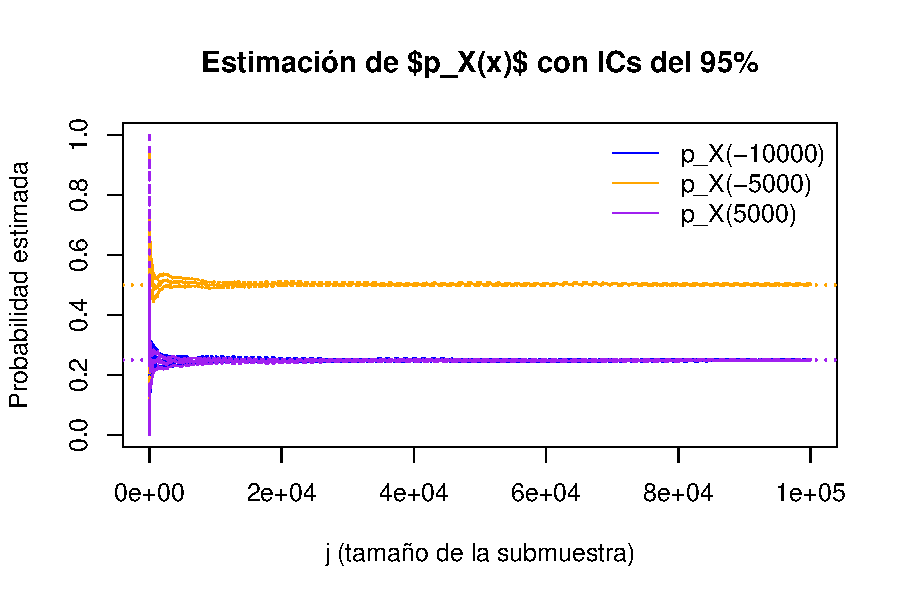
\includegraphics[width=\maxwidth]{figure/plot-probabilities-1} 
\end{knitrout}

Se observa cómo las probabilidades estimadas convergen a los valores reales a medida que aumenta el tamaño de muestra $j$, y cómo los intervalos de confianza se vuelven más estrechos.


\section{Bootstrap}

This exercise is based on the article Introduction to Bootstrapping in Statistics with an Example and the dataset body fat.csv that contains the body fat percentages of 92 adolescent girls. Generate a program that gives:

\subsection{An histogram of the sample data.}


\begin{knitrout}
\definecolor{shadecolor}{rgb}{0.969, 0.969, 0.969}\color{fgcolor}\begin{kframe}
\begin{alltt}
\hlcom{# Leer el archivo}
\hldef{fat_data} \hlkwb{<-} \hlkwd{read.csv}\hldef{(}\hlsng{"body_fat.csv"}\hldef{,} \hlkwc{stringsAsFactors} \hldef{=} \hlnum{FALSE}\hldef{)}

\hlcom{# Verifica el nombre exacto de la columna}
\hlkwd{colnames}\hldef{(fat_data)} \hlkwb{<-} \hlkwd{trimws}\hldef{(}\hlkwd{colnames}\hldef{(fat_data))}  \hlcom{# Eliminar espacios en el nombre}
\hldef{columna_objetivo} \hlkwb{<-} \hlkwd{colnames}\hldef{(fat_data)[}\hlnum{1}\hldef{]}         \hlcom{# Obtener el nombre real}

\hlcom{# Convertir a numérico por si acaso}
\hldef{fat_data[[columna_objetivo]]} \hlkwb{<-} \hlkwd{as.numeric}\hldef{(}\hlkwd{trimws}\hldef{(fat_data[[columna_objetivo]]))}

\hlcom{# Histograma}
\hlkwd{hist}\hldef{(fat_data[[columna_objetivo]],}
     \hlkwc{main} \hldef{=} \hlsng{"Histograma del porcentaje de grasa corporal"}\hldef{,}
     \hlkwc{xlab} \hldef{=} \hlsng{"Body Fat (%)"}\hldef{,}
     \hlkwc{col} \hldef{=} \hlsng{"skyblue"}\hldef{,}
     \hlkwc{border} \hldef{=} \hlsng{"white"}\hldef{)}
\end{alltt}
\end{kframe}
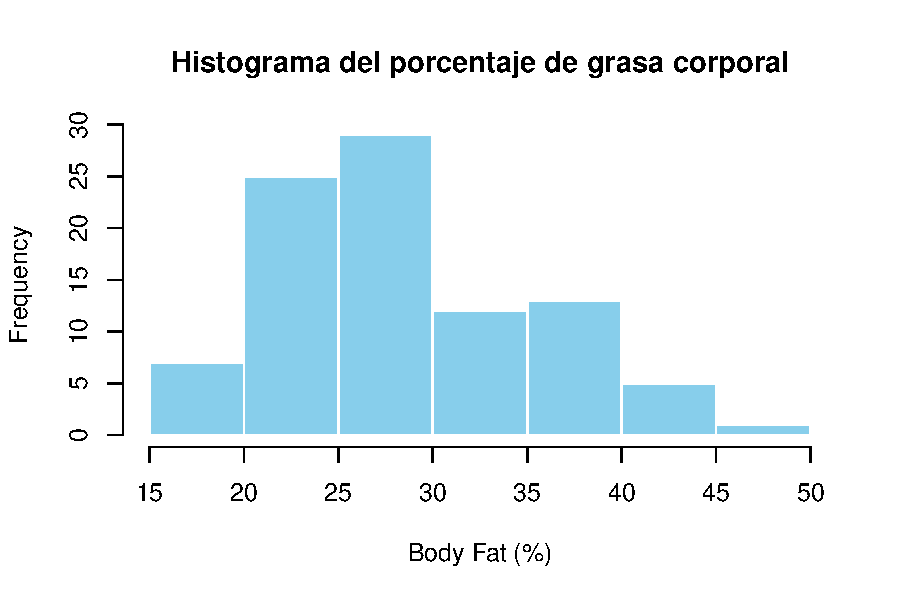
\includegraphics[width=\maxwidth]{figure/histograma-fat-1} 
\end{knitrout}


\subsection{The 95 \% confidence interval of the mean of the data from the traditional method (i.e., via the Central Limit Theorem).}


\begin{knitrout}
\definecolor{shadecolor}{rgb}{0.969, 0.969, 0.969}\color{fgcolor}\begin{kframe}
\begin{alltt}
\hlcom{# Estadísticas necesarias}
\hldef{media} \hlkwb{<-} \hlkwd{mean}\hldef{(fat_data[[columna_objetivo]],} \hlkwc{na.rm} \hldef{=} \hlnum{TRUE}\hldef{)}
\hldef{sd} \hlkwb{<-} \hlkwd{sd}\hldef{(fat_data[[columna_objetivo]],} \hlkwc{na.rm} \hldef{=} \hlnum{TRUE}\hldef{)}
\hldef{n} \hlkwb{<-} \hlkwd{sum}\hldef{(}\hlopt{!}\hlkwd{is.na}\hldef{(fat_data[[columna_objetivo]]))}  \hlcom{# número de datos no NA}

\hlcom{# Cálculo del error estándar}
\hldef{se} \hlkwb{<-} \hldef{sd} \hlopt{/} \hlkwd{sqrt}\hldef{(n)}

\hlcom{# Intervalo de confianza del 95%}
\hldef{alpha} \hlkwb{<-} \hlnum{0.05}
\hldef{z} \hlkwb{<-} \hlkwd{qnorm}\hldef{(}\hlnum{1} \hlopt{-} \hldef{alpha}\hlopt{/}\hlnum{2}\hldef{)}  \hlcom{# valor crítico Z para 95%}
\hldef{li} \hlkwb{<-} \hldef{media} \hlopt{-} \hldef{z} \hlopt{*} \hldef{se}
\hldef{ls} \hlkwb{<-} \hldef{media} \hlopt{+} \hldef{z} \hlopt{*} \hldef{se}

\hlcom{# Mostrar resultado}
\hlkwd{cat}\hldef{(}\hlkwd{sprintf}\hldef{(}\hlsng{"The 95%% confidence interval for the mean is: [%.2f, %.2f]"}\hldef{, li, ls))}
\end{alltt}
\begin{verbatim}
## The 95% confidence interval for the mean is: [27.14, 29.99]
\end{verbatim}
\end{kframe}
\end{knitrout}

Como se puede apreciar en el programa, hay un 95\% de confianza para que la media esté en el intervalo $[27.1370357, 29.9933991]$.

\subsection{A number of 500 bootstrapped samples from the original dataset, with 92 observations each.}


\begin{knitrout}
\definecolor{shadecolor}{rgb}{0.969, 0.969, 0.969}\color{fgcolor}\begin{kframe}
\begin{alltt}
\hlcom{# Vector original limpio}
\hldef{original_data} \hlkwb{<-} \hlkwd{na.omit}\hldef{(fat_data[[columna_objetivo]])}
\hldef{n} \hlkwb{<-} \hlkwd{length}\hldef{(original_data)}

\hlcom{# Generar 500 muestras bootstrap}
\hldef{bootstrap_samples} \hlkwb{<-} \hlkwd{replicate}\hldef{(}\hlnum{500}\hldef{,} \hlkwd{sample}\hldef{(original_data,} \hlkwc{size} \hldef{= n,}
                    \hlkwc{replace} \hldef{=} \hlnum{TRUE}\hldef{),} \hlkwc{simplify} \hldef{=} \hlnum{FALSE}\hldef{)}
\end{alltt}
\end{kframe}
\end{knitrout}

Este código utiliza la función \lstinline|replicate()| para repetir la operación 500 veces, la función \lstinline|sample()| toma una muestra con reemplazo del tamaño de 92.

\subsection{An histogram of the means of each bootstrapped sample.}

\begin{knitrout}
\definecolor{shadecolor}{rgb}{0.969, 0.969, 0.969}\color{fgcolor}\begin{kframe}
\begin{alltt}
\hlcom{# Calcular la media de cada muestra bootstrap}
\hldef{bootstrap_means} \hlkwb{<-} \hlkwd{sapply}\hldef{(bootstrap_samples, mean)}

\hlcom{# Histograma de las medias}
\hlkwd{hist}\hldef{(bootstrap_means,}
     \hlkwc{main} \hldef{=} \hlsng{"Histograma de medias de muestras bootstrap"}\hldef{,}
     \hlkwc{xlab} \hldef{=} \hlsng{"Media del % de grasa corporal"}\hldef{,}
     \hlkwc{col} \hldef{=} \hlsng{"lightgreen"}\hldef{,}
     \hlkwc{border} \hldef{=} \hlsng{"white"}\hldef{,}
     \hlkwc{probability} \hldef{=} \hlnum{TRUE}\hldef{)}  \hlcom{# Importante: escala el eje y para densidades}

\hlcom{# Parámetros de la normal}
\hldef{mean_boot} \hlkwb{<-} \hlkwd{mean}\hldef{(bootstrap_means)}
\hldef{sd_boot} \hlkwb{<-} \hlkwd{sd}\hldef{(bootstrap_means)}

\hlcom{# Añadir curva de distribución normal}
\hlkwd{curve}\hldef{(}\hlkwd{dnorm}\hldef{(x,} \hlkwc{mean} \hldef{= mean_boot,} \hlkwc{sd} \hldef{= sd_boot),}
      \hlkwc{col} \hldef{=} \hlsng{"blue"}\hldef{,} \hlkwc{lwd} \hldef{=} \hlnum{2}\hldef{,} \hlkwc{add} \hldef{=} \hlnum{TRUE}\hldef{)}
\end{alltt}
\end{kframe}
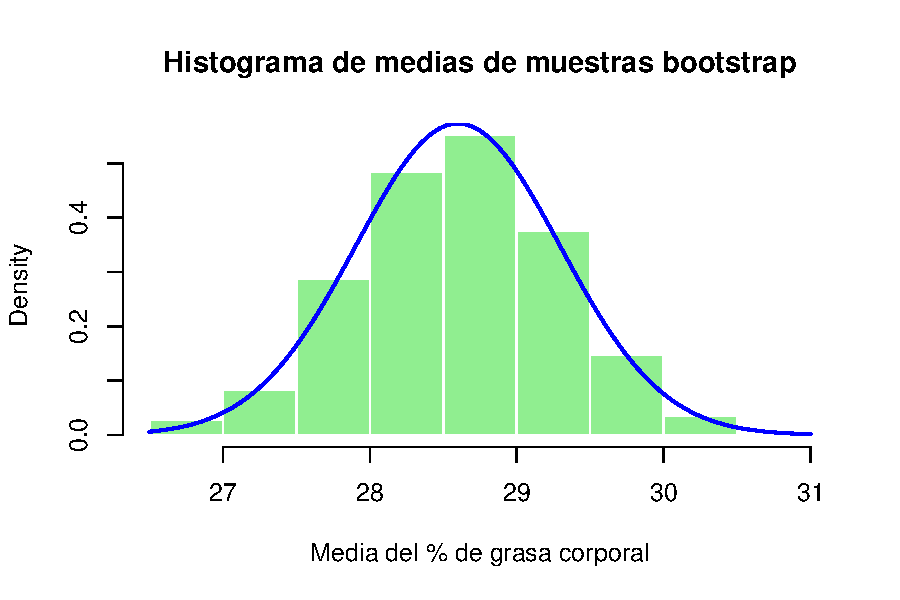
\includegraphics[width=\maxwidth]{figure/bootstrap-histogram-1} 
\end{knitrout}

Se puede ver como mas medias de muestras del bootstrap se asemejan a una distribución normal.

\subsection{A 95 \% bootstrapped confidence interval of the mean.}


\begin{knitrout}
\definecolor{shadecolor}{rgb}{0.969, 0.969, 0.969}\color{fgcolor}\begin{kframe}
\begin{alltt}
\hlcom{# Calcular intervalo de confianza bootstrap del 95%}
\hldef{bootstrap_ci} \hlkwb{<-} \hlkwd{quantile}\hldef{(bootstrap_means,} \hlkwc{probs} \hldef{=} \hlkwd{c}\hldef{(}\hlnum{0.025}\hldef{,} \hlnum{0.975}\hldef{))}

\hldef{bootstrap_ci}
\end{alltt}
\begin{verbatim}
##     2.5%    97.5% 
## 27.20592 29.90144
\end{verbatim}
\end{kframe}
\end{knitrout}


Entoncs, el 95\% del intervalo de confianza para la media es:

\[
\left[ 27.21,\; 29.9 \right]
\]


Con el método tradicional del teórema central del límite:

\[
  \left[ 27.14,\; 29.99 \right]
\]

Con el método \textit{bootstrap}

\[
  \left[ 27.21,\; 29.9 \right]
\]




\end{document}
